% ref:https://texample.net/media/tikz/examples/TEX/android.tex
% https://texample.net/tikz/examples/android/
\documentclass[border=10pt]{standalone}
\usepackage{amsmath}
\usepackage{amssymb}
\usepackage{tikz}
\usetikzlibrary{arrows.meta,calc}
\tikzset{%
  >={Stealth[width=1.5mm,length=2mm]},shorten >=2pt,
  % Specifications for style of nodes:
            base/.style = {rectangle, rounded corners, draw=black,
                           minimum width=2.5cm, minimum height=1cm,
                           text centered, font=\ttfamily},
  start/.style = {base, fill=blue!30},
       stop/.style = {base, fill=red!30},
         process/.style = {base,  fill=orange!15},
}

\DeclareMathOperator{\supp}{supp}
\DeclareMathOperator{\dist}{dist}
\DeclareMathOperator{\vol}{vol}
\DeclareMathOperator{\diag}{diag}
\DeclareMathOperator{\tr}{tr}
\DeclareMathOperator{\Img}{\operatorname{Im}}
\DeclareMathOperator{\Id}{\operatorname{Id}}
\DeclareMathOperator{\Rep}{\operatorname{Rep}}
\DeclareMathOperator{\Mod}{\operatorname{mod}}
\DeclareMathOperator{\Hom}{\operatorname{Hom}}
\DeclareMathOperator{\Ext}{\operatorname{Ext}}
\DeclareMathOperator{\Mor}{\operatorname{Mor}}
\DeclareMathOperator{\rad}{\operatorname{rad}}
\DeclareMathOperator{\ind}{\operatorname{ind}}
\DeclareMathOperator{\End}{\operatorname{End}}
\DeclareMathOperator{\Jac}{\operatorname{Jac}}
\DeclareMathOperator{\Spec}{\operatorname{Spec}}
\DeclareMathOperator{\Modup}{\overline{\operatorname{mod}}}
\DeclareMathOperator{\Moddown}{\underline{\operatorname{mod}}}
\DeclareMathOperator{\Homup}{\overline{\operatorname{Hom}}}
\DeclareMathOperator{\Homdown}{\underline{\operatorname{Hom}}}
\DeclareMathOperator{\gldim}{\operatorname{gl.dim}}
\DeclareMathOperator{\projdim}{\operatorname{proj.dim}}
\DeclareMathOperator{\injdim}{\operatorname{inj.dim}}
\DeclareMathOperator{\dimv}{\operatorname{\underline{\mathbf{dim}}}}


\DeclareMathOperator{\Flagd}{\operatorname{Flag}_{d}}
\DeclareMathOperator{\Flagdstr}{\operatorname{Flag}_{d,str}}
\newcommand{\Gr}{\operatorname{Gr}}
\newcommand{\Grr}{\operatorname{Gr}}
\newcommand{\Gralg}[1]{\operatorname{Gr}^{#1}}
\newcommand{\Grq}{\operatorname{Gr}^{KQ}}
\newcommand{\Flag}[1]{\operatorname{Flag}_{#1}}
\newcommand{\Flagstr}[1]{\operatorname{Flag}_{#1,str}}
\newcommand{\dimvec}[1]{\boldsymbol{#1}}
\newcommand{\ord}{\operatorname{ord}}
\newcommand{\orde}{\operatorname{ord}_e }
\newcommand{\representation}[2]{\genfrac{}{}{0pt}{3}{\phantom{000}#2\phantom{00}}{#1}}
\begin{document}    
% Drawing part, node distance is 1.5 cm and every node
% is prefilled with white background
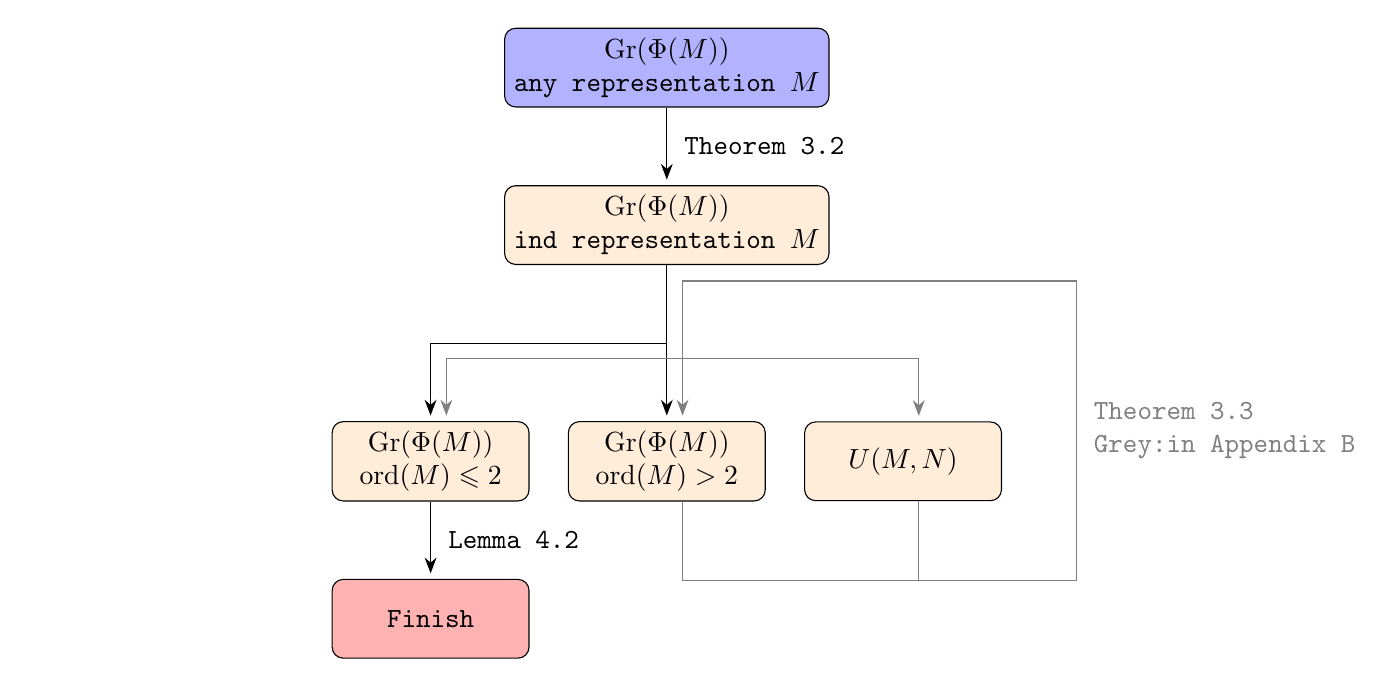
\begin{tikzpicture}[node distance=2cm, 
    every node/.style={fill=white, font=\sffamily}, align=center]
    \def\a{0.2}
    \def\b{-0.2}
  % Specification of nodes (position, etc.)
  \node (start)             [start]              {$\Grr(\Phi(M))$\\any representation $M$};
  \node (indrep)     [process, below of=start]          {$\Grr(\Phi(M))$\\ind representation $M$};
  \node (bigord)      [process, below of=indrep,yshift=-1cm]   {$\Grr(\Phi(M))$\\$\ord(M)>2$};
  \node (smallord)     [process, left of=bigord,xshift=-1cm]   {$\Grr(\Phi(M))$\\$\ord(M) \leqslant 2$};
  \node (diffe)      [process, right of=bigord,xshift=1cm]
                {$U(M,N)$};
  \node (stop) [stop, below of=smallord]
         {Finish};     
  \node (balance) [left of=smallord,xshift=-3cm]{};       
  % Specification of lines between nodes specified above
  % with aditional nodes for description 
\draw[->]   (start) --node [anchor=west,font=\ttfamily,xshift=1mm]{Theorem 3.2} (indrep);
\draw[->]   (indrep) -- (bigord);
\draw[->]   (smallord) --node [anchor=west,font=\ttfamily,xshift=1mm]{Lemma 4.2} (stop);
  \draw[->]      ($ (indrep)!.5!(bigord) $) -| (smallord);
   \draw[->,gray] ($ (bigord.south)+(\a,0)$) -- ++(0,-1) -- ++(5,0) --node[anchor=west,font=\ttfamily,xshift=1mm,align=left]
          {Theorem 3.3 \\ Grey:in Appendix B} ++(0,3.8) -- ++ (-5,0) --              
       ($(bigord.north)+(\a,0)$);
   \draw[->,gray] ($ (indrep)!.5!(bigord)+(\a,\b) $)-| ($ (smallord.north)+(\a,0) $);
   \draw[->,gray] ($ (indrep)!.5!(bigord)+(\a,\b) $)-| ($ (diffe.north)+(\a,0) $);
   \draw[-,gray,shorten >=0pt] ($ (diffe.south)+(\a,0) $) -- ++(0,-1);
  \end{tikzpicture}
\end{document}